\documentclass[diploma]{nanolab2015}

\usepackage{float}
\usepackage{subfigure}
\usepackage{booktabs}
\usepackage{dcolumn}
\usepackage[flushleft]{threeparttable}
\usepackage{makecell}
\usepackage{enumitem}
\usepackage{xparse}
\usepackage{svg}
\newcounter{descriptcount}
\NewDocumentEnvironment{enumdescript}{O{}}{%
    \setcounter{descriptcount}{0}%
    \renewcommand*\descriptionlabel[1]{%
      \stepcounter{descriptcount}%
      \normalfont\bfseries ##1%
    }%
    \description%
  }%
  {\enddescription}



\DeclareMathOperator{\Attention}{Attention}
\DeclareMathOperator{\softmax}{softmax}
\DeclareMathOperator{\ReLU}{ReLU}
\DeclareMathOperator{\MSE}{MSE}
\DeclareMathOperator{\AdamW}{AdamW}


\begin{document}
\begin{titlepage}
    \begin{center}
        \large
        Федеральное государственное бюджетное образовательное учреждение
        высшего образования «Московский государственный университет имени
        М.В.Ломоносова»

        МЕХАНИКО-МАТЕМАТИЧЕСКИЙ ФАКУЛЬТЕТ

        \textbf{Кафедра Математической теории интеллектуальных систем}\\
        \vspace{4cm}
        \textsc{\Large Курсовая работа}\\[5mm]
        {\LARGE Исследование нейросетевых методов построения кликовой модели для задач информационного поиска}
    \end{center}
    \vspace{3cm}
    \null

    \begin{flushright}
        \normalsize \underline{Выполнил:}
        \\студент 531 группы
        \\Зенин В. О.
        \\ \underline{\hspace{4cm}}
    \end{flushright}
    \vspace{1cm}

    \begin{flushright}
        \normalsize \underline{Научный руководитель:}
        \\к.ф.-м.н., н.с Половников В. С.
        \\ \underline{\hspace{4cm}}
    \end{flushright}

    \vfill
    \begin{center}
        \textbf{Москва - 2024}
    \end{center}
\end{titlepage}
\setcounter{page}{3}
\clearpage
\tableofcontents{}  % оглавление
\clearpage
\chapter{Введение}
Информационные системы занимают центральное место в обработке больших объемов данных. С увеличением количества информации важно разрабатывать методы поиска, которые обеспечат пользователям быстрое нахождение нужной информации. Одним из важных источников данных являются действия пользователей при поиске и работе с найденной информацией. Исследуя подобные данные можно извлекать из них различные признаки, способные улучшать качество поисковой системы и лучше удовлетворять потребности пользователя.

Одним из способов работы с такими данными являются кликовые модели, которые анализируют имеющуюся историю взаимодействия пользователей с результатами поисковой выдачи и помогают лучше понять, какие из показанных документов были более или менее полезны. Традиционные подходы к построению кликовых моделей включают в себя различные вероятностные методы, однако с развитием технологий машинного обучения все более актуальным становятся нейросетевые методы, обладающие в некоторых задачах высокой обобщающей способностью, позволяющей эффективно обрабатывать и анализировать сложные и многомерные данные.

Актуальность данной темы обусловлена как практическими потребностями, так и научным интересом. С одной стороны, улучшение алгоритмов информационного поиска напрямую влияет на качество пользовательского опыта и способность поисковых систем решать свою главную задачу по нахождению релевантного контента. С другой стороны, исследование нейросетевых методов в контексте кликовых моделей открывает новые горизонты в области машинного обучения и обработки больших данных.

Целью данной работы является изучение современных нейросетевых методов построения кликовых моделей и их применения в задачах информационного поиска. В работе будут рассмотрены как теоретические аспекты разработки таких моделей, так и практические примеры их внедрения и оценки эффективности. Мы проанализируем существующие подходы, выявим их преимущества и недостатки, а также предложим возможные направления для дальнейших исследований и улучшений.
\newpage
\section{Основные понятия и терминология}
\subsection{Поисковый запрос}
Поисковый запрос -- это текстовая строка, состоящая из ключевых слов, с которыми пользователь обращается к поисковой системе с целью удовлетворить свою информационную потребность. Основная задача информационного поиска это удовлетворение информационной потребности пользователя, которая выражена в составленном им запросе, посредством предоставления ему поисковой выдачи.
\subsection{Поисковая выдача}

Поисковая выдача по запросу $i$ -- это набор результатов $D_i$, которые поисковая система представляет пользователю в ответ на его поисковый запрос. Результаты включают ссылки на различные документы $(d_{i,1}, \dots, d_{i, M})$, которые поисковая система считает релевантными запросу пользователя.

Страницу результатов поиска, которую пользователь видит после ввода поискового запроса, принято называть серп, от SERP -- Search Engine Results Page. Серп обычно включает органические результаты (неоплаченные ссылки), платные результаты (рекламные ссылки), а также другие элементы, такие как изображения, видео, карты и фрагменты с ответами на вопросы.

\subsection{Пользовательская сессия}

Пользовательская сессия $S$ в контексте информационного поиска представляет собой последовательность взаимодействий пользователя с поисковой системой в течение определенного периода времени. В зависимости от контекста и целей анализа, можно выделить два типа сессий: сессии в широком смысле и сессии в узком смысле. Сессии в широком смысле будем обозначать $S$, сессии в узком смысле $s$, а множество всех сессий -- $\mathcal{S}$.

Сессия в широком смысле включает все действия пользователя, связанные с поиском информации, начиная с ввода первого поискового запроса $q_1$ и заканчивая завершением активности или истечением времени неактивности. В эту сессию входят все последующие перезапросы, изменения поисковых фраз, составляющие последовательность запросов $Q = \{q_i\}_{i=1}^N$, переходы по ссылкам, возвращения на страницу поиска, а также клики $C = \{c_{i,j}\}$ на результаты поиска, где $i$ -- порядковый номер запроса, к которому относятся клики по документам на позиции $j$. Клик кодируется бинарно $c_{i,j} \in \{0, 1\}$ -- 1 в случае клика и 0 иначе.

Каждая пользовательская сессия является тройкой: $(Q, C, D)$. По необходимости, для обозначения конкретной сессии из набора будем использовать индекс $k$. В случае сессий в широком смысле $\mathcal{S} = \{S_k\}_{k=1}^K$ каждой сессии $S_k$ соответствует тройка $(Q_{k} = \{q_{i,k}\}, C = \{c_{i,j,k}\}, D = \{d_{i,j,k}\})$. В случае сессий в узком смысле индекс $i$ можно опустить и писать соответственно $\mathcal{S} = \{s_k\}_{k=1}^K$ и $(Q_{k} = \{q_{k}\}, C = \{c_{j,k}\}, D = \{d_{j,k}\})$.

Сессия в узком смысле ограничивается взаимодействием пользователя в рамках одного конкретного поискового запроса $q$. В нее входят действия, связанные только с этим запросом.

Не трудно заметить, что сессия в широком смысле является последовательностью сессий в узком смысле и может быть на них разбита. Обратное же не верно, поскольку заданные в разное время пользовательские запросы могут не относится к удовлетворению его конкретной информационной потребности.

Действия пользователя зависят от типа показанного контента и не ограничиваются только кликами. Каждый тип принято называть вертикалью поиска. Например, если поисковая система показала видео в серпе, то гораздо важнее знать сколько времени пользователь его смотрел или досмотрел ли до конца.

\subsection{Релевантность}
Релевантность обозначает степень соответствия между поисковым запросом пользователя и предоставленными поисковой системой результатами. Чем выше степень соответствия между запросом и результатами, тем более релевантными считаются эти результаты для пользователя.

Иными словами, релевантность показывает, насколько хорошо результат поиска отвечает на запрос пользователя и удовлетворяет его информационные потребности. Это не только соответствие ключевым словам в запросе и содержанию документа, но и более общие факторы, такие как тематика, контекст и цель запроса.

Поисковая выдача формируется посредством работы алгоритма ранжирования, который анализирует признаки документов и упорядочивает их.

Для оценки релевантности составляется специальная инструкция, по которой эксперты (асессоры) оценивают пары запрос-документ и выставляют каждой из них оценку -- как правило это неотрицательное целое число.

Когда каждой паре запрос-документ сопоставлена такая численная оценка релеватности документа по этому запросу $rel$, можно оценить качество алгоритма ранжирования вычислив $DCG$ -- Discounted Cumulative Gain по формулам:
\begin{align}
    DCG@N = \sum_{j=1}^{N} \frac{rel_j}{log_2(j+1)} \label{dcg}
\end{align}
или
\begin{align}
    DCG_{exp}@N = \sum_{j=1}^{N} \frac{2^{rel_j} - 1}{log_2(j+1)} \label{dcg:exp}
\end{align}
где $N$ -- количество документов в выдаче, $j$ - позиция документа и $rel_j$ -- его релевантность. Можно заметить, что релевантные документы, оказавшиеся на последних позициях, дают малый вклад. Также как малый вклад дают и нерелевантные документы, оказавшиеся на первых позициях.

Существует способ нормализации $DCG$, приводящий её значения в диапазон от 0 до 1, заключающийся в вычислении $IDCG$ -- Ideal DCG. $IDCG$ это максимальное значение $DCG$ для данного запроса, но используя те же самые документы. Формула идентична (\ref{dcg}) или (\ref{dcg:exp}) (в зависимости от выбранной версии), за исключением того, что все документы должны быть отсортированы в порядке убывания их релевантности, т.е. при $j=1$ получается максимальная оценка релевантности из набора.
После чего нормализованный $DCG$, называющийся $nDCG$, вычисляется как отношение $DCG$ к соответствующему ему $IDCG$. Поскольку так оценивается выдача по одному запросу, для оценки по группе запросов берётся среднее арифметическое.

\subsection{Кликовая модель}
Кликовая модель в классическом понимании -- это статистическая модель, которая предсказывает вероятность того, что пользователь совершит клик -- $\mathcal{P}_{i,j} = P(c_{i,j} = 1)$ по определенному результату в поисковой выдаче, основываясь на исторических данных о кликах пользователей.

В отличии от других областей, например рекомендательных технологий, в поиске ключевым элементом является запрос и пользовательские сессии агрегируются по нему.

\subsection{Позиционная предвзятость}
Позиционная предвзятость -- это явление, при котором вероятность клика на определенный результат поисковой выдачи зависит не только от релевантности документа, но и от позиции этого документа в списке результатов. Результаты, которые находятся выше на странице выдачи, получают больше кликов независимо от их фактической релевантности, поскольку пользователи склонны кликать на первые несколько ссылок, не анализируя их подробно.


\subsection{Сравнение качества кликовых моделей}
Качество кликовых моделей можно оценивать комплексно с качеством поискового движка в целом, используя описанную метрику релевантности $DCG$. Однако, если требуется сравнить две модели между собой на одном и том же наборе данных, то для этого подходит перплексия:

\begin{align}
    PPL@j = 2^{-\frac{1}{N}\sum_{i=1}^{N}c_{i,j}\log\mathcal{P}_{i,j} + (1 - c_{i,j})\log(1 - \mathcal{P}_{i,j}) }
\end{align}

где $N$ -- количество запросов, $c$ -- метка фактически совершенного клика, а $\mathcal{P}$ -- предсказанная вероятность клика по документу на позиции $j$ по $i$-тому запросу.

Чем ниже перплексия, тем лучше алгоритм предсказывает тестовые данные. Чем выше, тем соответственно он хуже понимает зависимости в тренировочных данных, либо же данные разнородны. Поэтому перплексию принято использовать для сравнения нескольких алгоритмов или моделей машинного обучения на одинаковых наборах данных.

\section{Традиционные методы построения кликовых моделей}
В данном разделе мы последовательно рассмотрим некоторые методы, двигаясь от более простых к более сложным и каждый последующий метод будет учитывать недостатки предыдущего.
\subsection{CTR}
CTR (Click-Through Rate) — это метрика, используемая для измерения эффективности рекламы, поисковых результатов и других элементов, привлекающих клики. % метрика плохое слово, мы математики и это может сбить с толку

CTR рассчитывается как отношение количества кликов на определенный элемент (например, рекламное объявление или результат поиска) к количеству его показов. Формула для расчета CTR выглядит следующим образом:
\begin{align}
    CTR = \frac{clicks}{imps},
\end{align}
где $clicks = \sum_{i,j} c_{i,j} \cdot E_{i,j}$ -- количество кликов по документам $d_{i,j}$, которые пользователь видел ($E_{i,j}=1$) и $imps = \sum_{i,j}E_{i,j}$ -- количество показов этих документов пользователям в целом. Важно уточнить, что подразумевается под показом: пусть поисковый движок демонстрирует на странице 10 документов выдачи, но устройство пользователя, в самом простом примере, не позволяет отобразить их все сразу. Это значит, что, например, документ на позиции $j=10$ не виден $E_{i,10} = 0$ и пользователь априори не может на него кликнуть. Такие скрытые от пользователя документы не учитываются при вычислении $CTR$. То как пользователь обращает внимание на документы будет следовать некоторым гипотезам.

Для использования этой метрики в поиске важно, чтобы клики и показы документов происходили в рамках одного запроса. Таким образом, высокий CTR документа указывает на то, что пользователи чаще кликают по нему в контексте данного запроса, что предполагает его высокую релевантность и полезность. CTR может использоваться как дополнительный фактор в алгоритме ранжирования поисково движка, который, при прочих равных, стремился бы продвигать документы с высокой кликабельностью выше в выдаче.

Для сессий в широком смысле в качестве такого запроса можно использовать самый первый, исходя из предположения, что пользователь совершает перезапросы с целью уточнить первоначальный и найти в конечном итоге то, что у него не получилось найти с первого раза. Поскольку сессия в широком смысле содержит в себе несколько сессий в узком смысле, то CTR можно считать и по каждой такой сессии с уникальным запросом.

CTR обладает рядом существенных недостатков, среди самых важных можно выделить два: неустойчивость перед позиционной предвзятостью и злоупотреблением привлекательными заголовками. В первом случае высокий CTR будут получать документы на первых позициях в выдаче вне зависимости от их фактической релевантности. Во втором -- пользователя может заинтересовать непосредственно заголовок, в то время как сам документ покажется ему бесполезным и он быстро завершит его просмотр.

\subsection{ClickRank}
Данных метод применяется к сессиям в широком смысле и позволяет учесть время, которое пользователь проводит в документе.

Документами являются страницы в сети Интернет, переход на которых осуществляется кликом по странице в поисковой выдаче.
Пусть у нас имеется набор сессий в широком смысле $\mathcal{S} = \{S_k\}_{k=1}^K$. Каждой сессии из этого набора соответствует последовательность кликов $C_k$. Длиной сессии $n_k$ называется количество событий в $S_k$, в данном случае это количество кликов, т.е. $n_k = |C_k|$.

Документы из всех выдач внутри $S_k$ обозначим за $D_k = \{d_{k,p}\}_{p=1}^{|D_k|}$ -- их порядок в серпах не важен, поэтому мы можем рассматривать все документы в одном множестве опустив индексы $i,j$.
Стоит отметить, что $|C_k|$ в данном методе может быть больше $|D_k|$, поскольку пользователь может совершать клики в одни и те же документы многократно.

Каждый клик необходимо дополнить его индексом в последовательность кликов, а также можно избавиться от указания на принадлежность сессии в узком смысле, т.е. вместо индексов $i,j$ имеем: $C_k = (c_{k,p,r})$, где $r \in \{1, \dots, n_k\}$ и $p \in \{1, \dots, |D_k|\}$.

Каждой сессии $S_k$ установим в соответствие запрос $q_1 \in Q_k \in S_k$ и обозначим его $q_k$. Тогда локальный ClickRank \cite{clickrank} документа $d_{k,p}$ в сессии $S_k$ вычисляется следующим образом:
\begin{align}
    ClickRank(d_{k,p}, S_k) = \sum_{r=1}^{n_k} c_{k, p, r} \cdot w_r(r, n_k) \cdot w_t(k,p,r)
\end{align}

Весовая функция $w_r$ отвечает за порядок клика:
\begin{align}
    w_r(r, n_k) = \frac{2(n_k + 1 - r)}{n_k(n_k + 1)}
\end{align}

Функция является монотонно убывающей по $r$, что позволяет ей давать больший вес для кликнутых ранее документов. Поскольку пользователи кликают на документы из начала серпа раньше, данный метод не борется с позиционной предвзятостью. Однако он позволяет учитывать проводимое время посредством второй весовой функции $w_t$, которая отвечает за проведенное на странице время:
\begin{align}
    w_t(k,p,r) = (1 - e^{-\lambda_1 t_d(k,p,r)})e^{-\lambda_2 t_l(k,p,r)}
\end{align}

где $t_d(k,p,r)$ -- время, проведенное на странице $d_{k,p}$ после клика $c_{k,p,r}$ (для удобства оно может быть некоторым образом нормализовано, а способ нормализации лучше выбирать исходя из природы данных и подбирать, используя кросс-валидацию), а $t_l(k,p,r)$ -- время загрузки этой страницы страницы (часто можно положить его равным нулю, исходя из предположения, что пользователь проводит на странице намного больше времени, чем она загружается). Коэффициенты $\lambda_1$ и $\lambda_2$ также являются гиперпараметрами и могут быть подобраны под конкретные данные.

Также стоит отметить, что весовая функция для проводимого времени достаточно гибкая и зависит от предполагаемого распределения проводимого времени на странице. В приведенной формуле используется предположения о распределение Пуассона, но на некоторых данных лучшие результаты может показать, например, распределение Вейбулла.

Как правило, если пользователь завершил сессию на просмотре какого-то документа и не вернулся в поиск, то нельзя достоверно установить проведенное время. Это вынуждает нас предполагать, что оно бесконечно и, соответственно, последний кликнутый пользователем документ самый важный. Зачастую это не так, поскольку пользователь мог не найти удовлетворяющего его информационную потребность контента вовсе, что и послужило мотивом для завершения сессии.

Для нужд поиска необходимо агрегировать ClickRank. Способ агрегации выбирается под нужды конкретной задачи, например, можно вычислить позапросный ClickRank документа -- для этого достаточно суммарный ClickRank документа по сессиям с одинаковым первым запросом $q_k$ поделить на количество кликов, совершенных в данный документ по этому запросу.

Метод позволяет алгоритму ранжирования поднимать выше документы, на которые пользователи чаще кликают и где проводят больше всего времени.

Clickrank, как правило, не вычисляется для более поздних запросов в сессии по той причине, что если пользователь нашел по ним релевантную для себя информацию, то эти запросы уже достаточно точны и для поискового движка не составляет труда найти хорошие документы. Улучшать ранжирование нужно по первому запросу, поскольку существование перезапросов доказывает неспособность поискового алгоритма найти релевантные документы по нему без поведенческой информации.

\subsection{DBN}
Dynamic Bayesian Network (DBN) представляет собой расширение байесовских сетей, которое учитывает временные зависимости между переменными. В контексте кликовых моделей для задач информационного поиска DBN используется для моделирования последовательности кликов пользователя на результаты поиска, а временная зависимость представляет собой предположение о том, что пользователь просматривает результаты поисковой выдачи от первого к последнему, последовательно обращая внимание на каждый документ и некоторым образом с ним взаимодействуя.

Модель на основе DBN учитывает \cite{DBN}, что вероятность клика на результат поиска зависит от его позиции в выдаче. Также модель принимает во внимание вероятность того, что пользователь в принципе заметит и решит кликнуть на документ в выдаче, а после -- продолжит просмотр других результатов.

Модель задается уравнениями:
\begin{align}
    A_j = 1, E_j = 1                  & \Leftrightarrow C_j = 1 \label{dbn:1} \\
    P(A_j = 1)                        & = a_u                  \label{dbn:2}  \\
    P(S_j = 1| C_j = 1)               & = s_u                   \label{dbn:3} \\
    C_j = 0                           & \Rightarrow S_j = 0 \label{dbn:4}     \\
    S_j = 1                           & \Rightarrow E_{j+1} = 0 \label{dbn:5} \\
    P(E_{j+1} = 1 | E_j = 1, S_j = 0) & = \gamma                \label{dbn:6} \\
    E_j = 0                           & \Rightarrow E_{j+1} = 0 \label{dbn:7}
\end{align}


где $E, A, C, S$ -- случайные события:
\begin{itemize}
    \item $E_j$: заметил ли пользователь документ на позиции $j$
    \item $A_j$: привлек ли данный документ его внимание
    \item $C_j$: кликнул ли он на этот документ
    \item $S_j$: была ли удовлетворена информационная потребность пользователя
\end{itemize}
Тогда уравнения можно интерпретировать следующим образом:
\begin{itemize}
    \item (\ref{dbn:1}): Пользователь кликает на документ тогда и только тогда, когда он его заметил и тот привлек его внимание
    \item (\ref{dbn:2}): Привлекательность документа зависит только от него самого (не зависит от, например, позиции)
    \item (\ref{dbn:3}): Удовлетворенность пользователя кликнутым документом имеет некоторую вероятность
    \item (\ref{dbn:4}): Если пользователь не кликнул на документ, то его информационная потребность не была удовлетворена этим документом
    \item (\ref{dbn:5}): Если же документ $j$ удовлетворил пользователя, то он не замечает следующего за ним документа
    \item (\ref{dbn:6}): С некоторой вероятностью пользователь продолжит просмотр выдачи и заметит следующий документ, если остался не удовлетворен предыдущим
    \item (\ref{dbn:7}): Если пользователь не заметил документ, то и все последующие он не заметит
\end{itemize}

Вероятности $a_u$ и $s_u$ полагаются равными нулю и являются, по мере обновления, результатом обучения такой модели на исторических данных при заданной вероятности $\gamma$, которая, в свою очередь, уже является гиперпараметром и требует определения. Обычно её можно подобрать максимизируя $CTR$ документа на первой позиции. У авторов подхода лучшие результаты получаются при $\gamma = 0.9$, но простое предположение о $\gamma = 1$ приводит к результатам не сильно хуже, позволяя, при этом, упростить вычисления.

Используя для вычисления сессии всех пользователей, задавший определенный запрос, $a_u$ и $s_u$ каждого документа по данному запросу можно использовать далее как признаки для модели ранжирования.

Данный метод нивелирует описанные в других методах недостатки и является широко используемым не только в поиске, но и, например, в рекомендациях: ключевым отличием является то, что в поиске оценка $\gamma$ одинакова для всех пользователей, в то время как в рекомендациях -- каждый пользователь может иметь свою оценку.

Также DBN не учитывает реальную последовательность пользовательских действий: если пользователь кликнул по двум документам, причем первый клик пришелся на документ с большей позицией, то для модели всё будет ровно наоборот. Предположение о том, что пользователь просматривает документы исключительно сверху вниз и по порядку достаточно строгое.

\section{A Graph-Enhanced Click Model for Web Search}
Не составляет труда реализовать алгоритм машинного обучения, который бы решал задачу регрессии, предсказывая вероятность клика, если в качестве данных использовать различные документные характеристики, а в качестве разметки $CTR$ документов из исторических данных или даже просто бинарный признак: наблюдался ли хоть раз клик; было ли количество кликов больше некоторого заранее фиксированного числа и тому подобные.

Однако, особенностью задачи построения кликовой модели является недоступность информации о документах, кроме той, как с ними взаимодействовали пользователи в имеющихся исторических данных.

Более того, эти данные крайне разрежены: например, в интернете существуют как минимум миллиарды различных веб-страниц и бесчисленное множество запросов, по которым эти страницы могут быть показаны, а статистика представлена лишь по очень ограниченному числу относительно популярных запросов.

До этого мы не касались проблемы холодного старта -- когда кликовой модели необходимо предоставить какую-либо оценку качества документа с точки зрения его способности заинтересовать и быть полезным пользователю по тому запросу, который никогда до этого не был задан и отсутствует в исторических данных. Тем не менее, GraphCM \cite{GraphCM} сочетает в себе преимущества описанных ранее классический моделей, эффективно работает с разреженными данными и борется с проблемой холодного старта. Опишем подробнее компоненты данной модели и их роли в построении результирующей кликовой модели.

\subsection{Представление данных}
В качестве данных у нас имеются сессии в широком смысле, содержащие несколько запросов и поисковых выдач по ним, а также клики. Построим для запросов следующий граф: вершинами будут запросы, а соединяющие их ребра подчиняются правилам:
\begin{itemize}
    \item между двумя вершинами есть ребро, если запросы, соответствующие этим вершинам, встретились в одной сессии
    \item ребра есть между всеми вершинами, если по соответствующим им запросам был клик в один и тот же документ
\end{itemize}

Для сессий в широком смысле принимается во внимание гипотеза, что запросы в них, так или иначе, связаны между собой и являются попыткой пользователя решить одну задачу. Это же и отражено в построенном графе: между собой связаны запросы, встречавшиеся в одном контексте и документы, которые удовлетворили информационную потребность пользователя.

Для документов строится похожий граф, где уже они будут вершинами, а правила для построения ребер следующие:
\begin{itemize}
    \item между двумя вершинами есть ребро, если документы, соответствующие этим вершинам, были представлены в выдаче по одному запросу
    \item ребра есть между всеми вершинами, если по соответствующим им документам были клики по одному и тому же запросу
\end{itemize}

Подобное представленные данных является первым шагом в решении проблемы холодного старта: если наш поисковый движок добавил в выдачу документ, ранее не встречавшийся в ней, но остальные документы уже есть в графе, то мы можем добавить этот новый документ в граф. Похожим образом это работает и для новых запросов: в простом случае, если это один из запросов в текущей сессии, в которой до этого были запросы из нашего графа, то не составляет труда его добавить и использовать имеющуюся информацию; в более сложном варианте можно установить похожесть с группой запросов по поисковой выдаче, при совпадении документов-кандидатов для дальнейшего ранжирования.

Оба графа будут использоваться для работы графовой нейронной сети с механизмом внимания \cite{GAT} в описываемых далее компонентах. Для каждого поданного на вход эмбеддинга запроса или документа при помощи Graph Attention Network строится новый эмбеддинг, содержащий в себе уже информацию из графа, а именно извлекаемую при помощи механизма внимания \cite{Attention} информацию о соседях.

\subsection{Attractiveness Estimator}
Ранее мы рассматривали гипотезу (\ref{dbn:1}), с которой работал метод на основе DBN и одним из результатов его работы было получение оценки привлекательности документа по данному запросу $a_u$. В GraphCM для получения подобной оценки используются подходы на основе нейронных сетей, а именно несколько компонент: для запроса, документа и кликов.

\subsubsection{Query Encoder}
Поскольку запросы представляют из себя некоторых текст, в общем случае для них уместно использовать подходы из NLP, однако для нашей задачи необходимо лишь различать между собой запросы, а для этого достаточно сопоставить каждому из них определенный идентификатор. Тогда при помощи one-hot кодирования каждый запрос представляется как вектор, по которым строятся эмбеддинги низкой размерности при помощи соответствующего слоя.

Далее для каждой сессии эмбеддинги всех запросов $q_i$ пропускаются через слои GAT, что позволяет обогатить их информацией о контексте из соседних в графе запросов. Такие обогащенные эмбеддинги пропускаются через GRU \cite{GRU}, в результате чего получается один вектор, содержащий в себе всю доступную информацию о запросной части сессии.

\subsubsection{Document Encoder}
Аналогично запросом, документам тоже достаточно иметь только некоторый идентификатор, из которого не составляет труда получить one-hot представление, а также эмбеддинг по нему.

Для документов через соответствующий им граф и GAT пропускаются все документы из всех серпов по всем запросам сессии. К каждому такому обогащенному эмбеддингу документа конкатенируются эмбеддинги клика, позиции и вертикали, соответствующие данному документу. После всё также пропускается через GRU и получается один вектор, который содержит теперь в себе уже всю информацию о документной и поведенческой частях сессии.

\subsubsection{Neighbor Interaction Module}
Предыдущие компоненты работали с запросами и документами независимо друг от друга. Текущая же служит для извлечения информации о взаимодействии между ними. Также если до этого мы использовали в механизме внимания векторы из одной части сессии, запросной или документной, изолированно, то теперь применяем его к пропущенным через соответствующе GAT вектор запроса $q_i$ и документов по нему $d_{i,j}$.

Полученные от каждой компоненты векторы конкатенируются в один, который пропускается через полносвязные слои и дает оценку привлекательности $\mathcal{A}_{i,j}$ документа $d_{i,j}$, если бы он оказался в выдаче по запросу ${q_i}$.

\subsection{Examination Predictor}
Принимая во внимание гипотезу, что пользователь продолжит обращать внимание на документы не из-за контента этих документов, а в результате своих действий с предыдущими документами, только эти данные и будут использоваться в текущей компоненте.

Для каждого запроса и каждого документа сессии необходимо сконкатенировать соответствующие им эмбеддинги позиции, вертикали и клика, после чего пропустить их через GRU и превратить в оценку вероятности $\mathcal{E}_{i,j}$ посредством линейного слоя и сигмоиды в конце.

\subsection{Click Predictor}
Для получения вероятности клика теперь необходимо скомбинировать между собой $\mathcal{A}_{i,j}$ и $\mathcal{E}_{i,j}$. Лучшие результаты показал вариант комбинации
\begin{align}
    c = \mathcal{E}^\alpha \times \mathcal{A}^\beta
\end{align}
где $\alpha$ и $\beta$ параметры модели и подбираются посредством её обучения.
\chapter{Основная часть}
Задачей данной работы будет попытка применить метод GraphCM к новым данными и сравнение качества полученной модели с DBN.
\section{Формальная постановка задачи}
Пусть нам даны сессии в узком смысле $\mathcal{S} = \{s_k\}_{k=1}^K$, то есть каждая сессия состоит из одного запроса $q_k$ и одной поисковой выдачи по этому запросу: $D_k = \{d_{j, k}\}_{j=1}^M$, где $M$ -- длина серпа. Все документы также принадлежат одному типу контента, т.е. их вертикали $v_{j, k}$ одинаковы $\forall \; \space i \in \{1, \dots, K\} \subset \mathbb{N}, \; j \in \{1, \dots, M\} \subset \mathbb{N}$. Различные сессии могут иметь одинаковые запросы. Выдача по одинаковым запросам может быть разной.

Пусть также даны исторические данные, содержащие информацию о пользовательских действиях, а именно для каждой сессии $s_k$ имеется последовательность кликов $C_k = \{c_{j,k}\}_{j=1}^{M-1}$.

Необходимо обучить модель предсказывать, будет ли по запросу $q_k$ кликнут документ $d_{M, k}$, т.е. предсказать значение $c_{M, k} \in \{0, 1\}$.

\section{Данные}
В качестве данных будем использовать \href{https://github.com/agcr/vk-msu-ir-course-spring-2024/blob/055b4329ad60466c238044d3d1d16d2b9c9764d9/seminars/6-behaviour-ranking/iphone-20240201.tsv.gz}{суточные сессии ВК Видео пользователей устройств на операционной системе ios} \cite{vkds}. Идентичность вертикали обеспечивается тем, что все документы являются видеороликами.

Всего имеется 425951 сессий, каждая строка представляет собой одну сессию, содержащую:

\begin{enumerate}
    \item уникальный идентификатор сессии
    \item идентификатор запроса: равенство идентификаторов означает идентичность запросов, но не влечет за собой идентичность серпов
    \item позиции кликнутых документов: позиции упорядочены и не отражают последовать действий пользователя
    \item идентификаторы документов поисковой выдачи: равенство идентификаторов означает идентичность ссылок на документы в сети Интернет, но не гарантирует идентичности контента, расположенного по этим ссылкам.
\end{enumerate}

Максимальная длина серпа в датасете $M = 40$, мы же ограничимся $M = 10$. Данное решение мотивировано тем, что именно такая длина серпа использовалась авторами GraphCM. Использование серпов большей длины возможно, но затрудняет эксперименты: во-первых, клики за пределами первой десятки документов достаточно редки и, во-вторых, многие поисковые движки стараются показать максимально релевантный контент на своей первой странице выдачи из 10 документов.

Таким образом в результате имеем 165250 уникальных запросов и 1015096 уникальных документов.

\subsection{Обучающее и тестовое множества}
В общем случае разбиение на обучающее и тестовое множества можно выполнять по идентификаторам сессий так, чтобы в соответствующих множествах они не пересекались. В данной работе будет использован этот подход: 80\% всех сессий поступит на обучение и по 10\% -- будут использованы для валидации и теста. Однако можно использовать и другие методы:
\begin{itemize}
    \item Разбиение по времени сессии (как для временных рядов), которое гарантирует, что время сессий в тестовом множестве не меньше времени сессий из обучающего.
    \item Разбиение по запросам, которое дает непересекающиеся запросы в множествах. Этот подход позволяет оценить как себя ведет модель с проблемой холодного старта.
\end{itemize}

\section{Методы}
\subsection{DBN}
В качестве модели на основе DBN воспользуемся публично доступной реализацией \cite{dbngithub}, соответствующей сформулированным во введении уравнениям.

Для работы с ней наш датасет достаточно конвертировать: разбить каждую строку на $N+1$ строк, где $N$ -- количество кликов в сессии и первая строка соответствует запросу. Приводя к такому формату данные сессии в узком смысле мы получаем их в формате записи сессий в широком смысле, с которыми работает данная библиотека. Однако никакой дополнительной информацией сессии не обогащаются, потому считать их сессиями в широком смысле нельзя.

\subsection{GraphCM}
Поскольку мы будем работать с сессиями в узком смысле, то в графе для запросов ребра будут только между теми запросами, по которым был клик в один и тот же документ. Таким образом, информации внутри сессии становится меньше. Слой GRU также будет получать только один эмбеддинг и, фактически, не обогатит его дополнительной информацией.

Также у нас одна вертикаль, поэтому её эмбеддинг будет константным, а меняться будут только эмбеддинги кликов и позиций.

\bigbreak

В обоих методах принимается гипотеза, что пользователи просматривают серп от начала до конца, последовательно обращая внимание на каждый документ. Таким образом, не имеет значения, в какой последовательности в действительности были совершены клики, с точки зрения обеих моделей пользователи кликали на документы по их порядку в серпе.
\section{Эксперимент}
Для DBN не требуется подбирать гиперпараметры, поскольку качество модели от них слабо зависит. Однако для GraphCM, как и для любой другой нейросети, необходимо подобрать оптимальные значения, чтобы не допустить переобучения модели.

Обучение GraphCM выполнялось на графическом процессоре Radeon\textsuperscript{\texttrademark} RX 7800 XT с использованием набора библиотек AMD ROCm\textsuperscript{\texttrademark} 6.1. Архитектура реализована при помощи библиотек PyTorch 2.4 и PyTorch Geometric.
\subsection{Подбор параметров}
Использование GraphCM с лучшими параметрами для других датасетов приводило к переобучению, что достаточно обоснованно из-за различий в количестве данных, их природе и организации:
\begin{itemize}
    \item меньшее количество документов при сохранении достаточно большого размера эмбеддингов позволяет модели запомнить все документы и не приобрести обобщающей способности
    \item аналогично для запросов: вообще говоря, количество уникальных запросов в сессиях в широком смысле больше, чем в сессиях в узком смысле, т.к. перезапросы довольно уникальны и редко повторяются в сессиях даже с одним начальным запросом
\end{itemize}

Параметры перебирались в заданных диапазонах (таблица \ref{table:params}) при помощи фреймворка \href{https://optuna.org/}{optuna}. Обученные модели сравнивались на валидационном множестве по величине функции ошибки (бинарная кросс-энтропия). Задание для оптимизации -- подобрать параметры минимизирующие ошибку.

\begin{table}[ht]
    \centering
    \caption{Параметры GraphCM}
    \label{table:params}
    \begin{tabular}{|l|l|l|}
        \thead{\bf Параметр}        & \thead{\bf Диапазон} & \thead{\bf Лучшее значение} \\
        \midrule\midrule
        \texttt{num\char`_steps}    & [2000, 20000]        & 6400                        \\
        \texttt{batch\char`_size}   & $2^{[6, 10]}$        & 128                         \\
        \texttt{hidden\char`_size}  & $2^{[3, 7]}$         & 32                          \\
        \texttt{embed\char`_size}   & $2^{[3, 7]}$         & 128                         \\
        \texttt{dropout\char`_rate} & [0.2, 0.5]           & 0.45
    \end{tabular}
\end{table}

Метод градиентного спуска -- Adam, коэффициент регуляризации $0.5$, начальный коэффициент скорости обучения $10^{-3}$, уменьшающийся вдвое, когда перплексия модели на валидации 6 раз становилась больше минимальной.
\subsection{Результаты}
Оптимальные параметры по результатам 100 экспериментов перечислены в таблице \ref{table:params}. На рисунке \ref{pic1} изображен результат процесса перебора параметров, по которому можно судить об их оптимальности.

\begin{figure}[t]
    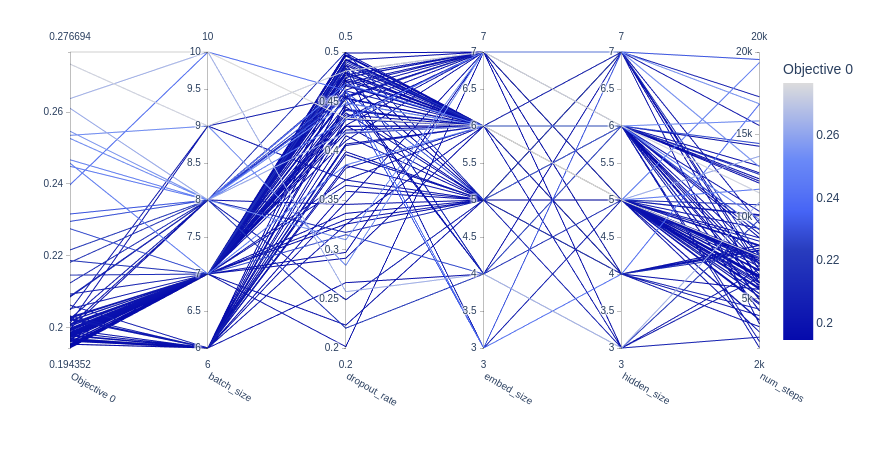
\includegraphics[scale=0.55]{./assets/optuna-params.png}
    \caption{Взаимосвязь параметров GraphCM. Objective 0 -- цель оптимизации (бинарная кросс-энтропия на валидационном множестве). Более плотные и насыщенные линии указывают на более перспективные значения параметров.}
    \label{pic1}
\end{figure}

Перплексия на тестовом множестве обученных моделей указана в таблице \ref{table:results}. Модели обучались на идентичных тренировочных множествах. На рисунках \ref{pic2} и \ref{pic3} изображены графики зависимостей перплексии на валидационном и тестовом множествах с лучшими параметрами модели соответственно. Можно выделить следующие особенности:
\begin{itemize}
    \item кривые практически идентичны, что указывает на согласованность в распределении данных между множествами и обеспечивает корректную оценку поведения модели;
    \item после локального минимума значения перплексии между шагами 5000 и 6000 она растет и 6 раз оказывается больше минимума, что провоцирует уменьшение коэффициента скорости обучения и приводит к снижению перплексии до уровня ниже, чем до пиков. Более того, продолжение обучения данной модели приводит к дальнейшему уменьшению перплексии, но не существенно (в 3 порядке).
\end{itemize}

Обучение с одинаковыми параметрами несколько раз дает немного отличающиеся значения в пределах $5 \cdot 10^{-3}$, что приемлемо для вычислений на графическом процессоре.

\begin{figure}[ht]
    \caption{Зависимость перплексии от количества шагов на валидационном множестве.}
    \includesvg[width=1\textwidth]{./assets/valid_perplexity.svg}
    \label{pic2}
\end{figure}

\begin{figure}[ht]
    \caption{Зависимость перплексии от количества шагов на тестовом множестве.}
    \includesvg[width=1\textwidth]{./assets/test_perplexity.svg}
    \label{pic3}
\end{figure}

\begin{table}[ht]
    \centering
    \caption{Значение перплексии на идентичных наборах данных}
    \label{table:results}
    \begin{tabular}{|l|l|}
        \thead{\bf Модель} & \thead{\bf PPL} \\
        \midrule\midrule
        DBN                & 1.276           \\
        GraphCM            & \bf1.235
    \end{tabular}
\end{table}


\chapter{Заключение}
В результате проведенных экспериментов удалось обучить модель GraphCM, работающую с сессиями в узком смысле, превосходящую по качеству классическую модель на основе DBN. Это достижение особенно примечательно, учитывая, что сессии в узком смысле не включают перезапросы и, следовательно, не предоставляют достаточной внутрисессионной информации. Несмотря на это ограничение, модель GraphCM смогла превзойти DBN, что демонстрирует её высокую эффективность и способность обрабатывать и анализировать данные даже в условиях ограниченной информации о взаимосвязи запросов. Эти результаты подчеркивают потенциал нейросетевых методов и их превосходство над традиционными подходами в задачах информационного поиска.

В качестве направлений для дальнейших исследований можно отметить следующие:
\begin{itemize}
    \item использование иных поведенческих сигналов: в работе использовался датасет с видеороликами, их можно не только кликать, но также и смотреть. Сигналы можно менять или использовать вместе -- хотя просмотр и более сильный сигнал, кажется, что в паре с кликом он может показать себя лучше;
    \item обучения модели большого размера и эксперименты с вариантами формирования обучающего множества. Имея больше данных и время сессии можно исследовать, что дает лучшее качество: регулярное дообучение на новых данных или переобучение с нуля;
    \item использование с учетом асессорских оценок: авторы GraphCM продемонстрировали рост DCG на датасете TianGong-ST \cite{TianGong} с имеющимися оценками, однако в нем представлены сессии в широком смысле. Мы показали, что перплексия модели на основе нейронной сети ниже классического DBN также и на сессиях в узком смысле, однако не имели асессорских оценок, чтобы исследовать, как недостаток внутрисессионной информации сказывается на поисковом движке в целом
\end{itemize}


\begin{thebibliography}{00}
    \bibitem{clickrank}
    Guangyu Zhu and Gilad Mishne. 2012. ClickRank: Learning Session-Context Models to Enrich Web Search Ranking. ACM Trans. Web 6, 1, Article 1 (March 2012), 22 pages. https://doi.org/10.1145/2109205.2109206
    \bibitem{DBN}
    Olivier Chapelle and Ya Zhang. 2009. A dynamic bayesian network click model for web search ranking. In Proceedings of the 18th international conference on World wide web (WWW '09). Association for Computing Machinery, New York, NY, USA, 1-10. https://doi.org/10.1145/1526709.1526711
    \bibitem{GraphCM}
    Jianghao Lin, Weiwen Liu, Xinyi Dai, Weinan Zhang, Shuai Li, Ruiming Tang, Xiuqiang He, Jianye Hao, and Yong Yu. 2021. A Graph-Enhanced Click Model for Web Search. In Proceedings of the 44th International ACM SIGIR Conference on Research and Development in Information Retrieval (SIGIR '21). Association for Computing Machinery, New York, NY, USA, 1259-1268. https://doi.org/10.1145/3404835.3462895
    \bibitem{GAT}
    Veličković, P., Casanova, A., Liò, P., Cucurull, G., Romero, A., \& Bengio, Y. (2018). Graph attention networks. OpenReview.net. https://doi.org/10.17863/CAM.48429
    \bibitem{Attention}
    Ashish Vaswani, Noam Shazeer, Niki Parmar, Jakob Uszkoreit, Llion Jones, Aidan N. Gomez, Łukasz Kaiser, and Illia Polosukhin. 2017. Attention is all you need. In Proceedings of the 31st International Conference on Neural Information Processing Systems (NIPS'17). Curran Associates Inc., Red Hook, NY, USA, 6000-6010.
    \bibitem{GRU}
    Chung, J., Gulcehre, C., Cho, K., \& Bengio, Y. (2014). Empirical evaluation of gated recurrent neural networks on sequence modeling. In NIPS 2014 Workshop on Deep Learning, December 2014
    \bibitem{vkds}
    Информационный поиск, 2024. https://github.com/agcr/vk-msu-ir-course-spring-2024
    \bibitem{dbngithub}
    PyClick - Click Models for Web Search. https://github.com/markovi/PyClick/
    \bibitem{TianGong}
    Jia Chen, Jiaxin Mao, Yiqun Liu, Min Zhang, and Shaoping Ma. 2019. TianGong-ST: A New Dataset with Large-scale Refined Real-world Web Search Sessions. In Proceedings of the 28th ACM International Conference on Information and Knowledge Management (CIKM '19). Association for Computing Machinery, New York, NY, USA, 2485-2488. https://doi.org/10.1145/3357384.3358158
\end{thebibliography}

\end{document}
